\part*{Rappels sur les courbes param\'etr\'ees}
\Def{Espace affine}{Ensemble non vide $\varepsilon$ associé à un $\mathbb{R}$-espace vectoriel E et qui est une muni d'une loi interne $\tilde{+}:\varepsilon\times E\to\varepsilon$ vérifiant :
\begin{itemize}
\item $\forall P,Q\in\varepsilon,\ \exists!u\in E;\ Q=P\tilde{+}u$ (qu'on note en général $u=\overrightarrow{PQ}$).
\item Pour tout $P\in\varepsilon$ et $u,v\in\varepsilon$, $P\tilde{+}(u+v)=(P\tilde{+}u)\tilde{+}v$.
\end{itemize}}

\Def{Longueur d'arc}{Valeur de $L=\int_I \|f'(t)\| dt$}

\Def{Arcs paramétrés équivalents}{On dit que deux arcs paramétrés $(I,f)$ et $J,g)$ définis dans l'espace affine $\mathcal{A}(\mathbb{R}^n)$ sont $\mathcal{C}^k$-équivalents si $f$ et $g$ sont de classe $\mathcal{C}^k$ et s'il existe une application bijective $\phi:J\to I$ vérifiant :
\[\left\{\begin{array}{c c c c}
g&=&f\circ g & \\
\phi &\text{ et } \phi^{-1} &\text{ sont de classe } \mathcal{C}^k
\end{array}\right.\]}

\part{B-splines}
\section{Fonctions polynômiales par morceaux (dans le plan)}
\subsection{Position du problème et notation}

Soit un intervalle fermé borné $[a,b]\subset \mathbb{R}$. On se donne une suite $\tau$ telle que :
	\[a<\tau_1<...<\tau_{l-1}<b\]
Par commodité, on pose $\tau_0=a$ et $\tau_l=b$.\\
Sur tout intervale $[\tau_i, \tau_{i+1}]$, on a une représentation polynomiale.\\
On définit une suite $r=\{r_i\}_{i=1}^{l-1}$ telle que \[0\leq r_i\leq k\]
Chaque $r_i$ est associé à $\tau_i$. Par convention, on prendra $r_0=0$.\\
On veut qu'en $\tau_i$, la courbe représentative admette un raccord de classe $\mathcal{C}^{r_i-1}$. On prend comme notation le fait que $\mathcal{C}^{-1}$ n'implique aucune condition.\\
\Def{}{On définit désormais $\mathcal{P}^{k,\tau,r}$ comme l'ensemble des fonctions polynomiales par morceaux de degré inférieur ou égal à $k$ ayant des raccords de classe $\mathcal{C}^{r_i-1}$ en $\tau_i$.}

\Theo{}{\[\text{dim }\mathcal{P}^{k,\tau,r}=(k+1)l-\sum_{i=1}^{l-1} r_i\]
De plus, une base de $\mathcal{P}^{k,\tau,r}$ est :
	\[\{(X-\tau_i)^j_+\},\ i\in \{0,...,n-1\},\ j\in \{r_i,...,k\}\]
avec $(X-\tau_i)_+=(X-\tau_i)\mathds{1}_{\{X\geq \tau_i\}}$}

\begin{dem}
Sur $[\tau_i,\tau_{i+1}]$, on a un polynôme $P_i$ de degré $k$. Posons $f_{ij}=(X-\tau_i)^j\mathds{1}_{\{X\in[\tau_i, \tau_{i+1}]\}}$, $j\in\{0,...,k\}$.\\
Sur $[\tau_i, \tau_{i+1}]$, nous avons un espace de dimension $k+1$. Si on on n'a pas de conditions en $\tau_i$, on a un espace de dimension $(k+1)l$.\\
On a :
\[P_j=\sum_{j=0}^k a_{ij} f_{ij}\]
On doit calculer les $a_{ij}$ pour $i\in \{0,...,l\}$ et pour $j\in \{0,...,k\}$.\\
De plus, en $\tau_i$, on veut un raccord de classe $\mathcal{C}^{r_i-1}$.\\
\[\text{Sur } [\tau_{i-1}, \tau_i],\ P_{i-1}=\sum_{j=0}^k a_{i-1,j} f_{i-1,j}\]
\[\text{Sur } [\tau_i, \tau_{i+1}],\ P_i=\sum_{j=0}^k a_{i,j} f_{i,j}\]
On veut donc $P_{i-1}^{(q)}(\tau_i)=P_i^{(q)}(\tau_i)$, $q\in\{0,...,r_{i-1}\}$.
\begin{eqnarray*}
\text{Pour } q=0,\ a_{i0}&=&\phi_0(a_{i-1,0},...,a_{i-1,k})\\
\text{Pour } q=1,\ a_{i1}&=&\phi_1(a_{i-1,1},...,a_{i-1,k})\\
\vdots\\
\text{Pour } q=r_{i-1}, a_{ir_{i-1}}&=&\phi_{r_{i-1}}(a_{i-1,r_{i-1}},...,a_{i-1,k})\\
\end{eqnarray*}

Avec $\phi_i$ linéaire.\\
Ainsi, $\forall j\in\{0,...,r_{i-1}\}$, \[a_{ij}=\phi_{j}(a_{i-1,j},...,a_{i-1,k})\]
En conclusion, le nombre total de relations est : \[\sum_{i=0}^{l-1} r_i\]
d'où \[\text{dim } \mathcal{P}^{k,\tau,r}=(k+1)l-\sum_{i=0}^{l-1} r_i\]

\bigskip
Vérifions à présent que \[A=\{(X-\tau_i)^j_+\}_{\begin{array}{c} i \in \{0,...,l-1\} \\ j\in\{r_i,...,k\} \end{array}}\]
est bien une base de $\mathcal{P}^{k,\tau,r}$.
\begin{itemize}
	\item card$(A)=\sum_{i=0}^{l-1}(k+1-r_i) = l(k+1)-\sum_{i=0}^{l-1} r_i = \dim \mathcal{P}^{k,\tau,r}$
	\item Vérifions que $(X-\tau_i)_+^j\in\mathcal{P}^{k,\tau,r}$.\\
En effet, pour $j\leq k$ :
	\begin{itemize}
		\item Si $X\to \tau_i^-$, $(X-\tau_i)^j_+\to 0$.
		\item Si $X\to \tau_i^+$, $(X-\tau_i)^j_+\to 0$.
	\end{itemize}
	Pour $X>\tau_i$, \[\frac{\partial^l}{\partial X^l} (X-\tau_i)^j_+=j(j-1)...(j-l)(X-\tau_i)^{j-l}_+\]
	Pour $X=\tau_i$, on a 0 tant que $j-l>0$, donc $l\leq r_i-1$ (car $j\in\{r_i,...,k\}$)
	\item Posons $F(X)=\sum_{i,j} a_{ij}(X-\tau_i)^j_+=0$ pour montrer que la famille est bien libre.
	\begin{eqnarray*}
		F(\tau_0)=a_{00} &\Rightarrow& a_{00}=0\\
		F'(\tau_0)=a_{01} &\Rightarrow& a_{01}=0\\
		F''(\tau_0)=2a_{02} &\Rightarrow& a_{02}=0 \\
		\vdots \\
		F^{(k)}(\tau_0)=k!a_{0k} &\Rightarrow& a_{0k}=0
	\end{eqnarray*}
	De la même manière, on a $F^{(r_i)}(\tau_i)=r_i!a_{i,r_i}=0$.
\end{itemize}
\end{dem}

\subsection{Fonctions splines}
On se donne la suite $\tau=(\tau_i)_{i=0,...,p}$ et la suite $r=(r_i)_{i=0,...,l-1}$ avec $r_i=k$ $\forall i\in\{1,...,l-1\}$.\\
On note alors $\mathcal{P}^{k,\tau,r}=S^{k,\tau}$ espace des fonctions splines.
	\[\dim S^{k,\tau}=(k+1)l-k(l-1)=l+k\]
Pour $k=3$, on a l'espace des splines cubiques.\\
On cherche des fonctions $f$ telles que  $f\in\mathcal{C}^2([a,b])$ avec :
\[(C)\left| \begin{array}{c c c c}
f(\tau_i)&=&y_i & \forall i\in\{0,...,l\}\\
f'(a)&=&\alpha & \text{ donné}\\
f'(b)&=&\beta & \text{ donné}
\end{array}\right.\]

On note $E$ l'ensemble des fonctions $\phi\in\mathcal{C}^2([a,b])$ avec $\phi$ vérifiant les conditions $(C)$.
\Theo{}{Il existe une unique fonction $\phi\in S^{3,\tau}$ vérifiant les conditions $(C)$.}

\begin{dem}
Voir polycopié
\end{dem}

\underline{Remarque :} Si $k_i=\tau_{i+1}-\tau_i=k=cste$, alors \[B=\begin{pmatrix} 4 & 1 & 0 & \cdots & \cdots & \cdots & 0 \\ 1 & \ddots & \ddots & \ddots & & & \vdots \\ 0 & \ddots & \ddots & \ddots & \ddots & & \vdots \\ \vdots & \ddots & \ddots & \ddots & \ddots & \ddots & \vdots \\ \vdots &  & \ddots & \ddots & \ddots & \ddots & 0 \\ \vdots & & & \ddots & \ddots & \ddots & 1 \\ 0 & \cdots & \cdots & \cdots & 0 & 1 & 4 \end{pmatrix}\]

\Lem{}{On prend $\phi\in S^{3,\tau}$ vérifiant les conditions $(C)$. On prend $f\in E$. On pose $e=f-\phi$, erreur dans l'aproximation de $f$ par $\phi$. Alors :
\[\int_a^b e''(x)g(x)dx = 0\ \forall g\in S^{1,\tau}\]}

\begin{dem}
\begin{eqnarray*}
\int_a^b e''(x)g(x) dx &=&\sum_{i=0}^{l-1} \int_{\tau_i}^{\tau_{i+1}} e''(x)g(x) dx \\
			&=& \sum_{i=0}^{l-1} [e'(x)g(x)]_{\tau_i}^{\tau_{i+1}} - \sum_{i=0}^{l-1} \int_{\tau_i}^{\tau_{i+1}} e'(x)g'(x) dx 
\end{eqnarray*}
\begin{eqnarray*}
\sum_{i=0}^{l-1} [e'(x)g(x)]_{\tau_i}^{\tau_{i+1}}&=&e'(\tau_l)g(\tau_l) - e'(\tau_0)g(\tau_0) \\
						&=& 0-0 \\
						&=& 0
\end{eqnarray*}

$g\in S^{1,\tau}$, donc sur $[\tau_i,\tau_{i+1}]$, $g'(x)=\lambda_i$.
\begin{eqnarray*}
\int_a^b e''(x)g(x) dx &=& -\sum_{i=0}^{l-1} \lambda_i \int_{\tau_i}^{\tau_{i+1}} e'(x) dx \\
			&=& -\sum_{i=0}^{l-1} \lambda_i (e(\tau_{i+1})-e(\tau_i)) \\
			&=& 0
\end{eqnarray*}
car $e(\tau_i)=f(\tau_i)-\phi(\tau_i)=0$. 
\end{dem}

\Theo{}{Si $\phi\in S^{3,\tau}\cap E$ ($\phi$ unique), on a : 
\[\int_a^b (\phi''(t))^2 dt = \min_{f\in E} \int^b_a f''(t)^2 dt\]
$\phi$ est l'unique élément de $E$ satisfaisant le minimum.}

\begin{dem}
On pose $e=f-\phi$.
\[\int_a^b f''(t)^2dt = \int_a^b \phi''(t)^2 dt + 2\int_a^b \phi''(t)e''(t) dt + \int_a^b e''(t)^2 dt\]
$\phi \in S^{3,\tau}$, donc $\phi''\in S^{1,\tau}$. D'après le lemme précédent :
\[\int_a^b \phi''(t) e''(t) dt = 0\]

Par conséquent :
	\[\int_a^b f''(t)^2 dt \geq \int_a^b \phi''(t)^2 dt\]
avec égalité si et seulement si :
\[\int_a^b e''(t)^2 dt = 0\]
Comme $e''$ est continue, on en conclut que $e''=0$\\
Or, $e'(a)=e'(b)=0$ et $\forall i\in \{1,...,l-1\}$, $e(\tau_i)=0$, donc $e$ est identiquement nulle.\\
En conclusion, il existe donc une unique fonction $f$ de $E$ donnant le minimum : c'est $\phi \in S^{3,\tau}$.
\end{dem}

\subsection{Fonctions B-splines}

On considère l'espace vectoriel $\mathcal{P}^{k,\tau,r}$.
\begin{itemize}
	\item $k$ est quelconque
	\item les fonctions amettent des raccords de classe $\mathcal{C}^{r_i-1}$ en les $\tau_i$ avec $r_i\leq k$, $\forall i\in \{1,...,l-1\}$.
\end{itemize}

\subsubsection{Notations}
On considère dans $\mathbb{R}$ une suite de points $t_0,...,t_m$ tels que $t_i\leq t_{i+1}$ $\forall i\in\{0,...,m-1\}$, appelés n\oe uds.

\Def{multiplicité}{Si $s$ n\oe uds consécutifs $t_i$ sont confondus $(t_i=t_{i+1}=...=t_{i+s-1})$, on dit que le n\oe ud est de multiplicité $s$.}

D'autre part, on pose \[w_{ij}(x)=\frac{x-t_i}{t_{i+j}-t_i} \mathds{1}_{\{t_i<t_{i+1}\}}\]
Par convention, à chaque fois que nous écrivons une fraction dont le dénominateur est nul, il faudra l'interpréter comme étant nulle.

\subsubsection{Définition des B-splines}
Posons $t=(t_0,...,t_m)$.\\
Pour $x\in \mathbb{R}$, $0\leq i\leq m-k-1$, les fonctions $B_{i,k,t}$ notées aussi $B_{i,k}$ lorsque la suite $t$ est fixée, sont définies via la relation de récurrence sur $k$ suivante :
\[B_{i,0}(x)=\mathds{1}_{[t_i,t_{i+1}[}(x)\]
Pour $k\geq 1$ :
\[B_{i,k}(x)=w_{i,k}(x)B_{i,k-1}(x) + (1-w_{i+1,k}(x))B_{i+1,k-1}(x)\]

\bigskip
\underline{Remarque :} Si pour un indice $i$, $t_i=t_{i+1}=...=t_{i+k+1}$ (donc $t_i$ est un n\oe ud de multiplicité $\geq k+2$), alors on a $B_{i,k}\equiv 0$.

\Prop{}{Si $t_i$ est de multiplicité $k+2$, alors $B_{i,k}(x)=0$}

\begin{dem}
\[B_{i,k}(x)=w_{i,k}(x)B_{i,k-1}(x) + (1-w_{i+1,k}(x))B_{i+1,k-1}(x)\]
Or, $t_i=t_{i+1}=...=t_{i+k+1}$, donc on a $w_{i,k}(x)=0$ et $w_{i+1,k}(x)=0$. Par conséquent :
	\[B_{i,k}(x)=B_{i+1,k-1}(x)\]
et par une récurrence simple, on montre finalement que :
\[B_{i,k}(x)=....=B_{i+k,0}(x) = \mathds{1}_{[t_{i+k},t_{i+k+1}[}(x)\]
\end{dem}

On écarte dans toute la suite la possibilité d'avoir un n\oe ud de multiplicité $k+2$.

\Theo{}{\begin{enumerate}
\item $B_{i,k}$ est polynomiale par morceaux de degré $k$ (par récurrence)
\item $B_{i,k}(x)=0$ si $x\not\in [t_i, t_{i+k+1}[$. On appelle $[t_i,t_{i+k+1}[$ le support de $B_{i,k}$ (récurrence)
\item $B_{i,k}(x)>0$ si $x\in]t_i, t_{i+k+1}[$ (récurrence)\\
	$B_{i,k}(t_i)=0$ sauf si $t_i$ de multiplicité $k+1$, car alors $B_{i,k}(t_i)=1$
\item Soit $[a,b]\subset \mathbb{R}$ tel que $t_0,...,t_k<a$ et $t_{m-k},...,t_m\geq b$. 
\[\forall x\in [a,b[,\ \sum_{i=0}^{m-k-1} B_{i,k}(x)=1\]
\item Soit $x\in]t_i,t_{i+k+1}[$, alors :
	\[B_{i,k}(x)=1 \Leftrightarrow x=t_{i+1}=....=t_{i+k}\]
\item $B_{i,k}$ est continue à droite et même indéfiniment dérivable à droite.
\end{enumerate}}

\begin{dem}
\begin{enumerate}
\setcounter{enumi}{2}
\item Montrons que si $t_i$ est de multiplicité $k+1$, alors $B_{i,k}(t_i)=1$. \\
La relation de récurrence donne :
\[B_{i,k}(x)=w_{i,k}(x)B_{i,k-1}(x)+(1-w_{i+1,k}(x))B_{i+1,k-1}(x)\]
Comme $t_i=...=t_{i+k}$, on a :
	\[w_{i,k}(t_i)=0 \text{ et } w_{i+1,k}(t_i)=0\]
Par conséquent : 
\[B_{i,k}(t_i)=B_{i+1,k-1}(t_i)=B_{i+1,k-1}(t_{i+1})\]
et $t_{i+1}$ est de multiplicité $k$, donc d'après l'hypothèse de récurrence, $B_{i+1,k-1}(t_{i+1})=B_{i,k}(t_i)=1$

\bigskip
On traite désormais le cas où $t_i$ est de multiplicité $<k+1$.
\begin{itemize}
	\item Si $t_i<t_{i+1}$, de la relation de récurrence : 
		\[B_{i,k}(t_i)=\underbrace{w_{i,k}(t_i)}_{=0}B_{i,k-1}(t)+(1-w_{i+1,k}(t_i))\underbrace{B_{i+1,k-1}(t_i)}_{=0}\]
car $t_i\not\in[t_{i+1},t_{i+k+1}[$.
	\item Dans le cas général, $t_i$ est de multiplicité $k$. Donc $t_{i+1}$ est de multiplicité $k-1$. Dans ce cas critique : 
		\[B_{i,k}(t_i)=(1-w_{i+1,k}(t_i))B_{i+1,k-1}(t_i) = (1-w_{i+1,k}(t_i))\underbrace{B_{i+1,k-1}(t_{i+1})}_{=0}\]
d'après l'hypothèse de récurrence puisque $t_{i+1}$ est de multiplicité au plus $k-1$.
\end{itemize}

\item On procède par récurrence sur k. On sait que :
	\[B_{i,0}(x)=\mathds{1}_{[t_i,t_{i+1}[}(x)\]
On en déduit donc que 
	\[\sum_{i=0}^{m-1}B_{i,0}(x)=1 \text{ si } x\in[t_0,t_m[\]
Or, par hypothèse, $t_0\leq a$ et $t_m\geq b$. En conclusion, $\forall x\in [a,b[$ :
	\[\sum_{i=0}^{m-1} B_{i,0}(x)=1\]
Supposons la propriété vraie jusqu'au rang $k-1$ et démontrons alors que la propriété reste vraie au rang $k$.\\
Soit $x\in[a,b]$. Il existe donc $j$, $k\leq j\leq m-k-1$ tel que $x\in[t_j,t_{j+1}[$.\\
Le support de $B_{i,k}$ est $[t_i, t_{i+k+1}[$. Comment avoir $[t_i,t_{i+k+1}[\cap[t_j,t_{j+1}[\neq \emptyset$ ?
\[\left\{\begin{array}{c c c}
	j&<&i+k+1\\
	i&<&j+1
 \end{array}\right. \Rightarrow
 \left\{\begin{array}{c c c}
	j&\leq& i+k\\
	i&\leq& j
 \end{array}\right.\]

D'où \[\sum_{i=0}^{m-k-1}B_{i,k}(x)=\sum_{i=j-k}^j B_{i,k}(x)\]
En utilisant la relation de récurrence définissant $B_{i,k}$, on a :
\begin{eqnarray*}
	\sum_{i=j-k}^j B_{i,k}(x)&=&\sum_{i=j-k}^j w_{i,k}(x) B_{i,k-1}(x)+\sum_{i=j-k}^j (1-w_{i+1,k}(x))B_{i+1,k-1}(x)\\
				&=&\sum_{i=j-k}^j w_{i,k}(x)B_{i,k-1}(x)+\sum_{I=j-k+1}^{j+1} (1-w_{I,k}(x))B_{I,k-1}(x)\\
				&=&\sum_{I=j-k+1}^{j+1} B_{i,k-1}(x)+w_{j-k,k}(x)B_{j-k,k-1}(x)+w_{j+1,k}(x)B_{j+1,k-1}(x)
\end{eqnarray*}
Or, $B_{j-k,k-1}(x)=0$ car son support est $[t_{j-k},t_j[$ et $x\in[t_j,t_{j+1}[$. Pour la même raison, $B_{j+1,k-1}(x)=0$. Ainsi :
\begin{eqnarray*}
	\sum_{i=j-k}^j B_{i,k}(x)&=&\sum_{I=j-k+1}^j B_{I,k-1}(x) + \underbrace{B_{j+1,k-1}(x)}_{=0}\\
				&=& 1
\end{eqnarray*}
d'après l'hypothèse de récurrence.\\
D'après l'axiome de récurrence, on a pour tout $k$ :
	\[\sum_{i=0}^{m-k-1} B_{i,k}(x)=1\]
\end{enumerate}
\end{dem}

\Rem{}{Dans le cas où $t_{m-k}=...=t_m=b$, la formule 4 n'est valable que sur $[a,b[$. En effet, pour tout $i\in\{0,...,m-k-1\}$, on a $B_{i,k}(b)=0$. Pour avoir une formule valable sur $[a,b]$, on est amené par abus de langage à poser $B_{m-k-1,k}(b)=1$, ce qui rend la B-spline $B_{m-k-1,k}$ continue à gauche en b. On fera systématiquement cet abus.}

\Propo{}{Pour tout $k\geq 0$ et tout $x\in\mathbb{R}$, $B_{i,k}$ est dérivable à droite et l'on a :
	\[B_{i,k}'(x)=k\left[\frac{B_{i,k-1}(x)}{t_{i+k}-t_i}-\frac{B_{i+1,k-1}(x)}{t_{i+k+1}-t_{i+1}} \right]\]
avec la convention que l'on remplace par 0 un expression dont le dénominateur est nul.}

\subsection{Les B-Splines comme base de $\mathcal{P}^{k,\tau,r}$}
Voir papier distribué.
\Def{}{Soit $t_i$, $0\leq i\leq m$ une suite de points de $\mathbb{R}$ telle que $t_i\leq t_{i+1}$, k un entier positif ou nul, $[a,b]$ un intervalle tel que $t_k\leq a$ et $t_{m-k}\geq b$. On note $\mathcal{P}^{k,t}([a,b])$ ou simplement $\mathcal{P}^{k,t}$ l'espace vectoriel des fonctions polynômiales par morceaux sur $[a,b]$ de degré $\leq k$, avec raccords de classe $\mathcal{C}^{k-p_j}$ en $t_j$, si $t_j$ est n\oe ud de multiplicité $p_j$.\\
Par convention, un racord de classe $\mathcal{C}^{k-p_j}$ avec $k-p_j<0$ n'impose aucune condition en $t_j$.}

\Theo{}{Supposons que tous les n\oe uds soient de multiplicité $\leq k+1$, alors $\{B_{i,k,t}\}_{i=0}^{m-k-1=n-1}$ est une base de $\mathcal{P}^{k,\tau,r}=\mathcal{P}^{k,t}$.}

\subsection{Algorithmes de base pour les B-splines}
Soit \[S(x)=\sum_{i=0}^{n-1} a_i B_{i,k}(x)\]
un élément de $\mathcal{P}^{k,t}$. \\
On dira que $S$ est une fonction spline.\\
Les B-splines sont calculées à l'aide d'une suite de n\oe uds $t_0,...,t_m$ et définies sur $\mathbb{R}$.

\bigskip
Nous allons étudier 3 algorithmes :
\begin{itemize}
	\item L'algorithme dit "De Boor-Cox" ou de "De Casteljan" permettant d'évaluer $S$ en un point donné $\hat{x}$ de $[a,b]$
	\item L'algorithme permettant de calculer les coefficients de la déviée $S'$ par rapport aux $B_{i,k-1}$
	\item L'algorithme d'insertion d'un n\oe ud.
\end{itemize}

\subsubsection{Algorithme d'évaluation}
\Propo{}{Soit $\hat{x}\in[a,b]$ (donc $\hat{x}\geq t_k$). On a :
\begin{eqnarray*}
S(\hat{x})&=&\sum_{i=0}^{n-1} a_i^{(0)} B_{i,k}(\hat{x}) \\
	&=& \sum_{i=0}^{n-1} a_i^{(1)}(\hat{x}) B_{i,k-1}(\hat{x}) \\
	&\vdots& \\
	&=&\sum_{i=0}^{n-1} a_i^{(k)}(\hat{x}) B_{i,0}(\hat{x})
\end{eqnarray*}
avec \[\begin{array}{c c l c}
a_i^{(0)}&=& a_i, & \forall i\in\{0,...,n-1\} \\
a_i^{(r+1)}(\hat{x})= &=& w_{i,k-r}(\hat{x})a_i^{(r)}(\hat{x}) + (1-w_{i,k-r}(\hat{x}))a_{i-1}^{(r)}(\hat{x})
\end{array}\]}

\begin{dem}
\[S(\hat{x})=\sum_{i=0}^{n-1} a_i^{(0)} B_{i,k}(\hat{x})\]
\[B_{i,k}(\hat{x})=w_{i,k}(\hat{x}) B_{i,k-1}(\hat{x})+(1-w_{i+1,k}(\hat{x}) B_{i+1,k}(\hat{x})\]
Par conséquent :
\begin{eqnarray*}
S(\hat{x})&=&\sum_{i=0}^{n-1} a_i^{(0)} w_{i,k}(\hat{x})B_{i,k-1}(\hat{x})+\sum_{i=0}^{n-1} a_i^{(0)} (1-w_{i+1,k}(\hat{x})B_{i+1,k-1}(\hat{x})\\
	&=&\sum_{i=0}^{n-1} a_i^{(0)} w_{i,k}(\hat{x})B_{i,k-1}(\hat{x})+\sum_{I=0}^{n} a_{I-1}^{(0)} (1-w_{I,k}(\hat{x})B_{I,k-1}(\hat{x})\\
	&=&\sum_{i=1}^{n-1} \underbrace{(a_i^{(0)} w_{i,k}(\hat{x})+a_{i-1}^{(0)}(1-w_{i,k}(\hat{x})))}_{=a_i^{(1)}}B_{i,k-1}(\hat{x}) + a_0^{(0)}w_{0,k}(\hat{x})\underbrace{B_{0,k-1}(\hat{x})}_{=0 \text{ à cause du support}}+a_{n-1}^{(0)}(1-w_{n,k}(\hat{x}))\underbrace{B_{n,k}(\hat{x})}_{=0} \\
	&=&\sum_{i=1}^{n-1} a_i^{(1)} B_{i,k-1}(\hat{x})
\end{eqnarray*}
La démonstration se termine par une récurrence immédiate, analogue à ce calcul.
\end{dem}

Si on veut évaluer $S(\hat{x})$ pour $x\in[t_j,t_{j+1}[$, on a donc :
	\[S(\hat{x})=a_j^{(k)}(\hat{x})\]
puis $B_{j,0}$ est la fonction indicatrice de l'intervalle $[t_j,t_{j+1}[$. \\
Pour calculer $a_j^{(k)}(\hat{x})$, il suffit d'évaluer les $a_i^{(k)}$ pour $i\in\{j-k+r+1,...,j\}$, les autres $B_{i,k-r}(\hat{x})$ étant nuls puisque :
\begin{eqnarray*}
	S(\hat{x})&=&\sum_{i=j-k}^{j} a_i^{(0)} B_{i,k}(\hat{x})\\
		&=& \sum_{i=j-k+1}^{j} a_i^{(1)}(\hat{x}) B_{i,k-1}(\hat{x})\\
		&\vdots& \\
		&=&a_j^{(k)}(\hat{x})
\end{eqnarray*}
L'algorithme se présente donc sous forme triangulaire, chaque élément s'obtenant par combinaire convexe des deux éléments de la ligne supérieure qui sont au-dessus de lui.\\
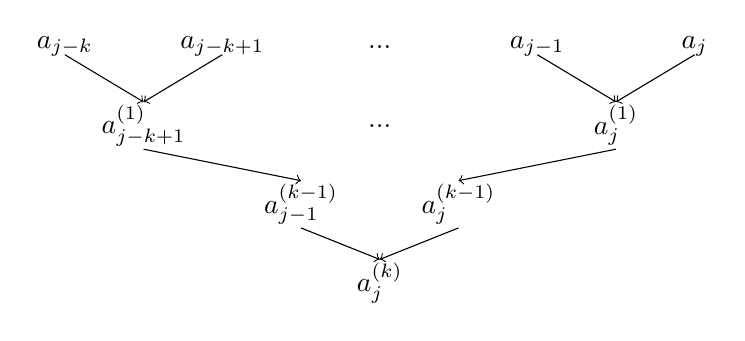
\begin{tikzpicture}
	\draw (1,3) node{$a_{j-k}$};
	\draw (3,3) node{$a_{j-k+1}$};
	\draw (5,3) node{...};
	\draw (7,3) node{$a_{j-1}$};
	\draw (9,3) node{$a_j$};
	\draw (2,2) node{$a_{j-k+1}^{(1)}$};
	\draw [->] (1,2.9)--(2,2.3);
	\draw [->] (3,2.9)--(2,2.3);
	\draw (5,2) node{...};
	\draw (8,2) node{$a_j^{(1)}$};
	\draw [->] (9,2.9)--(8,2.3);
	\draw [->] (7,2.9)--(8,2.3);
	\draw (4,1) node{$a_{j-1}^{(k-1)}$};
	\draw (6,1) node{$a_j^{(k-1)}$};
	\draw [->] (2,1.7)--(4,1.3);
	\draw [->] (8,1.7)--(6,1.3);
	\draw (5,0) node{$a_j^{(k)}$};
	\draw [->] (4,0.7)--(5,0.3);
	\draw [->] (6,0.7)--(5,0.3);
\end{tikzpicture}

\bigskip
\underline{Remarque :} \begin{enumerate}
	\item Cet algorithme est couteux en nombre d'opérations : il nécesite le calcul de $\frac{k(k+1)}{2}$ combinaisons convexes, et pour chaque combinaison, il faut :
	\begin{itemize}
		\item 2 multiplications
		\item 1 division
		\item 4 soustractions
	\end{itemize}
	soit un algorithme en $\sim3k^2$ opérations.
	\item Il a néanmoins plusieurs avantages : \begin{enumerate}
		\item Il est stable numériquement
		\item Le calcul des $w_{i,k-r}(\hat{x})$ est souvent très simple en pratique en particulier lorsque $\hat{x}$ et les n\oe uds $t_i$ sont entiers.
	\end{enumerate}
\end{enumerate}

Si on veut calculer la fonction $S$ en plusieurs points de $[t_j, t_{j+1}[$, on procède, en général, différemment.\\
On calcule une fois pour toute l'expression polynômiale de $S$ entre $t_j$ et $t_{j+1}$ :
	\[S(x)=\sum_{i=0}^k \frac{D^iS(t_j)}{i!} (x-t_j)^i\]
Avec $D^iS(t_j)$ les dérivées à droite évaluées formellement avec l'algorithme des dérivées ci-dessous. On évale $S(x)$ par la règle de Hörner ($\sim2k$ opérations).

\subsubsection{Algorithme des dérivées}
\Propo{}{Soit $S(x)$ défini précédemment. Alors la dérivée à droite $DS(x)$ est donnée par :
	\[DS(x)=\sum_{i=1}^{n-1} b_iB_{i,k-1}(x)\]
avec \[b_i=\left| \begin{array}{c c c} 
k\frac{a_i-a_{i-1}}{t_{i+k}-t_i} &\text{ si }& t_i<t_{i+k}\\
0 &\text{ sinon}
\end{array}\right.\]}

\begin{dem}
\begin{eqnarray*}
DS(x)&=&\sum_{i=0}^{n-1} a_i k \left[\frac{B_{i,k-1}(x)}{t_{i-k}-t_i} - \frac{B_{i+1,k+1}(x)}{t_{i+1+k}-t_{i+1}} \right] \\
	&=&\sum_{i=0}^{n-1} a_i k \frac{B_{i,k-1}(x)}{t_{i-k}-t_i} - \sum_{I=1}^{n}a_{I-1} k \frac{B_{I,k+1}(x)}{t_{I+k}-t_{I}}\\
	&=&\sum_{i=0}^{n-1} \underbrace{k \frac{a_i-a_{i-1}}{t_{i+k}-t_i}}_{=b} B_{i,k-1}(x) + ka_0\underbrace{\frac{B_{0,k-1}(x)}{t_k-t_0}}_{=0} - ka_{n-1}\underbrace{\frac{B_{n,k-1}(x)}{t_{n-k}-t_n}}_{=0}
\end{eqnarray*}
\end{dem}

\subsubsection{Algorithme d'insertion d'un n\oe ud}
Considérons $\{t_i\}$, $i\in\{0,...,m=n+k\}$. On obtient ainsi $B_{i,k,t}$, avec $i\in\{0,...,n-1\}$.\\
On ajoute $\hat{t}\leq t_{n-1}$ à cette suite. On considère donc une nouvelle suite $t'$ avec $t'=t\cup\{\hat t\}$ et $\{t_i'\},\ u\in\{0,...,n\}$.
\[\Rightarrow \hat{B}_{i,k,t'}, i\in\{0,...,n\}\]

\Propo{}{\[S(x)=\sum_{i=0}^{n-1} a_iB_{i,k,t}(x) = \sum_{i=0}^n \hat{a}_i B_{i,k,t'}(x) \]
avec \[\hat{a}_i=\left| \begin{array}{c c c} 
a_i&\text{ si }& t_{i+k}<\hat t\\
w_{i,k}(\hat t)a_i+(1-w_{i,k}(\hat t))a_{i-1} &\text{ si }& t_i<\hat t<t_{i+k}\\
a_{i-1} &\text{ si }& \hat t\leq t_i
\end{array}\right.\]}
